\documentclass[12pt]{beamer}
\usetheme{Pittsburgh}
%\setbeamertemplate{frametitle}[default][left]
% Somehow rightbound frame titles - change it?
\usepackage[utf8]{inputenc}
\usepackage[english]{babel}
\usepackage{amsmath}
\usepackage{amsfonts}
\usepackage{amssymb}
\usepackage{graphicx}
\usepackage{xcolor}
\usepackage{tikz}
\author{Sebastian Valet, Johannes Walter}
\title{Human Capital Investments and Expectations about Career and Family}
\date{July 7, 2020}
%\setbeamercovered{transparent} 
%\setbeamertemplate{navigation symbols}{} 
%\logo{} 
%\institute{} 
%\date{} 
%\subject{} 
\begin{document}

\begin{frame}
\titlepage
\end{frame}

%\begin{frame}
%\tableofcontents
%\end{frame}

% Summary: Research question and design
\begin{frame}{Summary I}
    \framesubtitle{Research questions and design}
        \begin{itemize}
            \item What do students believe about the consequences of their education choices?
            \item How do students sort into majors?
            \item Novel: what role do family variables play in such choices?
        \end{itemize}
    \vspace{0.5cm}
        \begin{itemize}
            \item Survey with undergraduate students at NYU on perceptions about consequences of educational choices
            \item Specifically: choice of a major
            \item Follow-up survey after six years
        \end{itemize}
\end{frame}

% Summary: Results
\begin{frame}{Summary II}
    \framesubtitle{Results}
    \begin{itemize}
        \item Students believe in importance of consequences for own earnings and family life
        \item Particularly women, major choice also corresponds to different rates and timing of marriage and fertility
        \item Belief about marriage market "return" to higher earning majors
        \item Ex-ante beliefs are systematically related to educational choices and ex-post realized outcomes
    \end{itemize}
\end{frame}

% Model of beliefs and realized choices
\begin{frame}{Model I}
    \framesubtitle{Human capital investment under uncertainty}
    \begin{itemize}
        \item Expected utility for human capital choice at time $\tau$: 
        $$ E_{i,\tau}(V_k) = \sum_{t = \tau + 1}^{T} \beta^{t - \tau}  \int u_t(X) \; dG_{i,\tau}(X|k,t) $$
        \item with discount rate $beta$ and outcome $X$ for all subsequent periods given a human capital investment $k$
        \item $G_{i,\tau}(X|k,t)$ is the belief distribution about the outcome given human capital investments $k$
    \end{itemize}   
\end{frame}

% Belief distribution
\begin{frame}{Model II}
    \framesubtitle{Belief distribution $G_{i,\tau}(X|k,t)$}
    \begin{itemize}
        \item Survey design elicits beliefs $G_{i,\tau}(X|k,t)$ about the choice of a major
        \item Belief distrubtions have four characteristics:
        \begin{itemize}
            \item reflect individual \textit{uncertainty}
            \item are \textit{heterogenous}
            \item can be \textit{incorrect}
            \item can evolve over time due to \textit{learning}
        \end{itemize}
        \item Natural limitation: elicitation of degree of uncertainty \textcolor{red}{ask Jogibär if put here; also how do they elicit?}
    \end{itemize}
\end{frame}

% Effects of Human Capital Choices
\begin{frame}{Model III}
    \framesubtitle{Different effects of human capital choices}
    \begin{itemize}
        \item Ex-ante individual differences in beliefs
        $$ \Delta_{G,i}(k,k') = G_i(X|k,t) - G_i(X|k',t) $$
        \item Ex-post individual differences in potential outcomes
        $$ \Delta_{F,i}(k,k') = F_i(X|k,t) - F_i(X|k',t) $$
        \item Ex-post individual differences realized outcomes
        $$ \Delta_{H}(k,k') = H(X|k,t) - H(X|k',t) $$ \\
        with $H(X|k,t) = \frac{1}{M_k} \sum_{t \in \Omega_k} F_i(k = k^*,t)$
    \end{itemize}
    
\end{frame}

\begin{frame}{Data}
    \begin{itemize}
        \item Survey among NYU undergraduate students in 2010
        \item Beliefs about earnings, earnings growth, earnings uncertainty, marriage, spousal earnings, fertility and labor supply
        \item Questions conditioned on ages 23, 30 and 45
        \item Sample consists of 493 individuals
        \item Follow-up survey 6 years later
    \end{itemize}
\end{frame}

% Here Table 1 in the appendix for descriptive statistics
\begin{frame}{Beliefs and Human Capital Choices I}
    \begin{itemize}
        \item Do beliefs actually influence intended and actual decisions?
        \item Intended major and actual major are outcome variables in the analysis
    \end{itemize}  
\end{frame}

\begin{frame}{Beliefs and Human Capital Choices II}
     \begin{center}
        \begin{tikzpicture}
            \node[anchor=south west,inner sep=0] at (0,0) {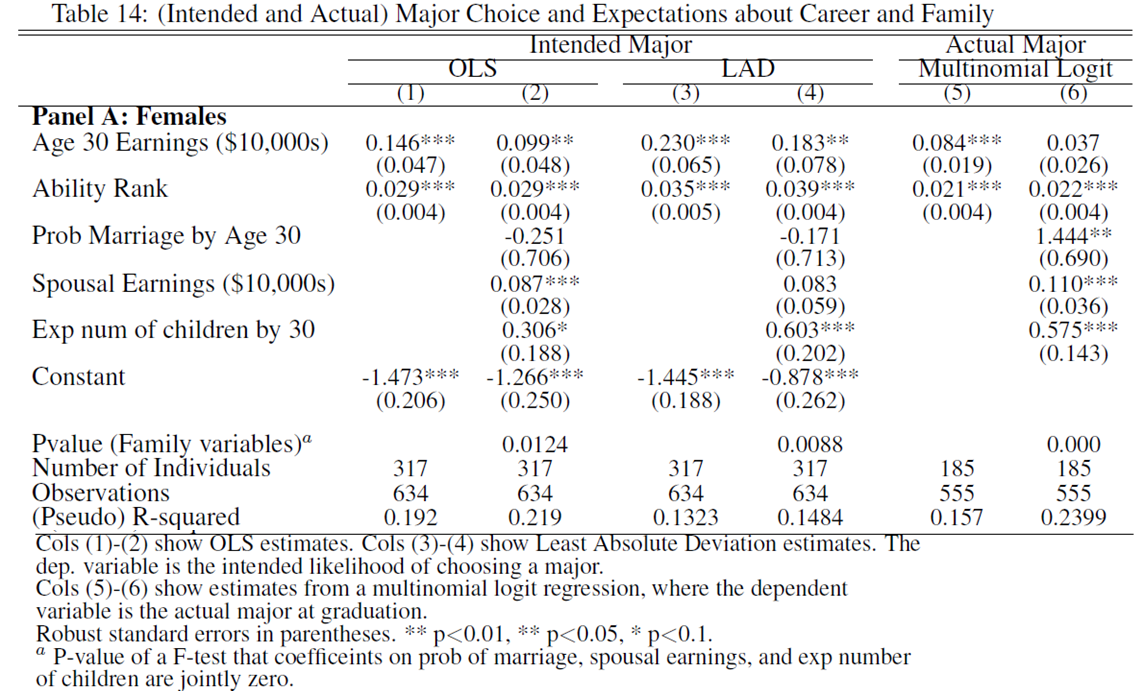
\includegraphics[scale = 0.35]{Graphs/Table14-female.png}};
            \draw<2>[red,ultra thick,rounded corners] (3.3,4.3) rectangle (8.0, 5.3);
            \draw<3>[red,ultra thick,rounded corners] (4.4,3) rectangle (8.0, 4.4);
            \draw<4>[red,ultra thick,rounded corners] (8.4,3) rectangle (10.5, 5.3);
        \end{tikzpicture}
    \end{center}
\end{frame}

\begin{frame}{Beliefs and Human Capital Choices III}
    \begin{center}
        \begin{tikzpicture}
            \node[anchor=south west,inner sep=0] at (0,0) {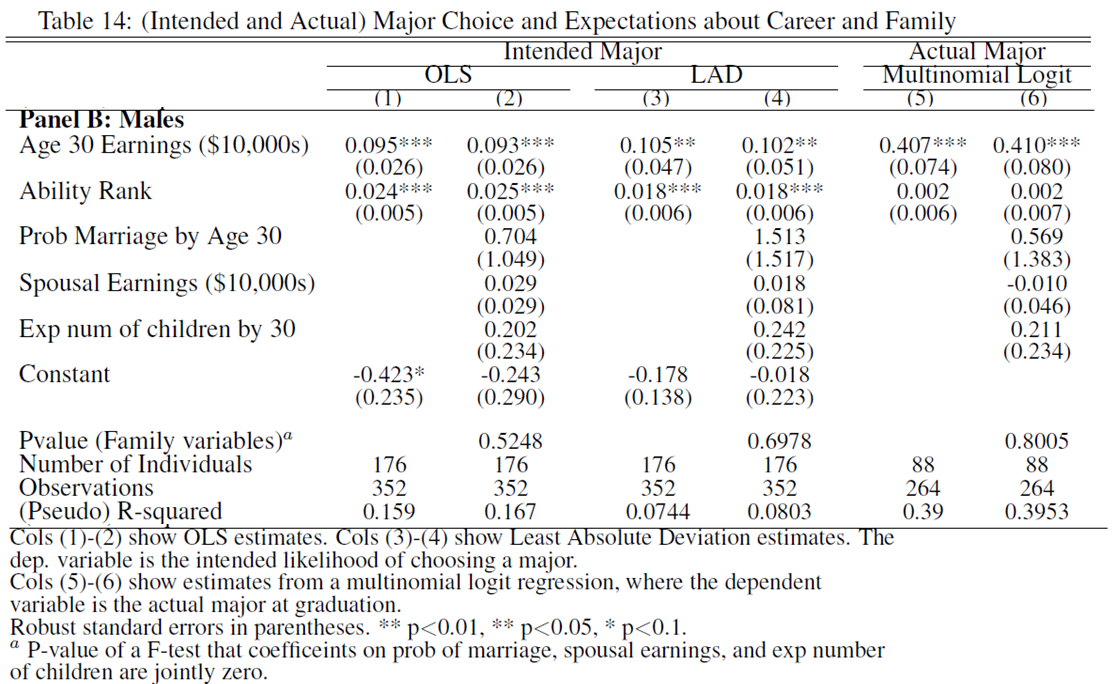
\includegraphics[scale = 0.35]{Graphs/Table14-male.png}};
            \draw<2>[red,ultra thick,rounded corners] (3.1,4.2) rectangle (7.8, 5.2);
            \draw<3>[red,ultra thick,rounded corners] (4.1,2.9) rectangle (7.8, 5.2);
            \draw<4>[red,ultra thick,rounded corners] (7.9,2.9) rectangle (10.3, 5.2);  
        \end{tikzpicture}
    \end{center}
\end{frame}


\begin{frame}{Beliefs and Realized Outcomes I}
    \framesubtitle{Follow-up survey}
    \begin{itemize}
        \item Follow-up survey six years after the initial survey
        \item 274 out of the initial 493 respondents participated
        \item Average age of respondent is 25
        \item Provides some evidence for the "quality" of the expectations data
        \item Respondents are not reminded of their initial answers
    \end{itemize}
    
\end{frame}

\begin{frame}{Beliefs and Realized Outcomes II}
    \framesubtitle{Population descriptive statistics}
    \begin{itemize}
        \item No statistically significant differences in expectations for earnings and working full-time
        \item 18\% of females expected to work part-time, but only 9\% in reality
        \item Large significant differences in expectations about marriage
        \item Significant difference in females expectations about partner's earnings: expectation 64.000 vs. realization 85.000
    \end{itemize}
\end{frame}

\begin{frame}{Beliefs and Realized Outcomes III}
    \framesubtitle{Individual-level relationshp}
    \begin{tikzpicture}
        \node[anchor=south west,inner sep=0] at (0,0) {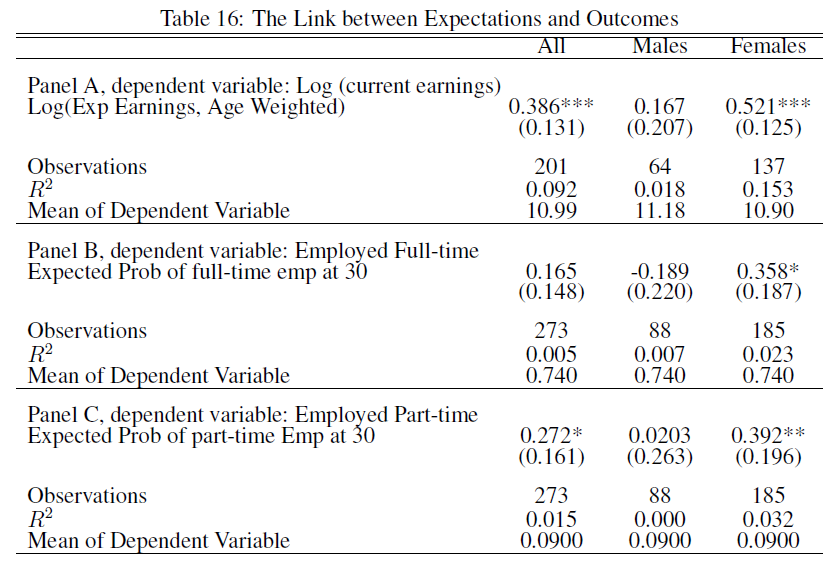
\includegraphics[scale = 0.35]{Graphs/Table17-earnings.png}};
        \draw<2>[red,ultra thick,rounded corners] (3.3,4.3) rectangle (8.0, 5.3);
    \end{tikzpicture}
\end{frame}

% These sildes can probably go in the appendix
% We should probably skip this section entirely? In the appendix?
\begin{frame}{Current Population Characteristics I}
    \begin{itemize}
        \item Earnings, employment, and marriage data for the US population using the 2009
        \item Not suited for causal inference; needs not reflect the student's beliefs
        \item Data from older cohort; includes not only high-ability participants
        \item But data is suited to document that career and family outcomes differ by educational choices in observational data
    \end{itemize}
\end{frame}

% Earnings Beliefs: Earnings Levels
\begin{frame}{Earnings Beliefs}
    \framesubtitle{Earnings Levels} 
    \begin{itemize}
        \item Male students believe to earn more than female students at each age
        \item All students believe to see rapid growth in earnings
        \item Students believe to see substantially smaller earning growth if they don't major in science/business
        \item Perceived gender gap is largest in science/business and at later stages
    \end{itemize}
\end{frame}

% Earnings Beliefs: Earnings Returns
\begin{frame}{Earnings Beliefs}
    \framesubtitle{Earnings Returns and Earnings Growth} 
    \begin{itemize}
        \item Should I make go more into details here?
    \end{itemize}
\end{frame}

% Beliefs about Marriage and Spousal Characteristics
%Layout needs to be changed on this slide
\begin{frame}{Beliefs about Marriage and Spousal Characteristics}
    \framesubtitle{} 
    \begin{itemize}
        \item Recent theory predicts that investment in education generates returns in the marriage market
        \item Probabilities: 
        \begin{itemize}
            \item Women belief they are slightly more likely to be married at younger ages, but no difference at age 45
            \item Students believe they are less likely to be married without a degree
        \end{itemize}
        \item Potential Spouse's Earnings
        \begin{itemize}
            \item Men expect lower, women expect higher earnings for their potential Spouse
            \item Students believe graduating in science or business relative to humanities or no degree will result in a higher earning spouse
            \item There is evidence for assortative mating by education
        \end{itemize}
    \end{itemize}
\end{frame}

% Beliefs about Fertility
\begin{frame}{Beliefs about Fertility}
    \framesubtitle{} 
    \begin{itemize}
        \item Conditioned on ages 30 and 45
        \item Men and women believe that completing a science or business degree rather than a degree in the humanities would reduce their expected number of children at age 30
        \item In contrast, completing a degree relative to no degree doubles expected number of children
        \item Students believe major choice has a larger effect on the timing of fertility rather than on the level
    \end{itemize}
\end{frame}

% Beliefs about Future Labor Supply
\begin{frame}{Beliefs about Future Labor Supply}
    \framesubtitle{} 
    \begin{itemize}
        \item Students believe their human capital choice will substantially affect their future employment
        \item Beliefs about working full-time is higher for males and higher for science/business degree relative to a degree in humanities
        \item Students' beliefs about their age 30 labor supply conditional on future expected marital status:
        \item Male students beliefs about future labor supply vary little by marital status, female students believe to work less when married
    \end{itemize}
\end{frame}

\begin{frame}{Future Research}
    \framesubtitle{} 
    \begin{itemize}
        \item Run follow-up surveys when students realize outcomes at ages 30 and 45
        \item Choice of participants casts doubt on external validity: extend the Sample
        \item Study elicits student's beliefs, but does not uncover the reasons for these beliefs
        \item Stated beliefs are not consequential
    \end{itemize}
\end{frame}

%Current Pop stats
\begin{frame}{Current Population Characteristics II}
    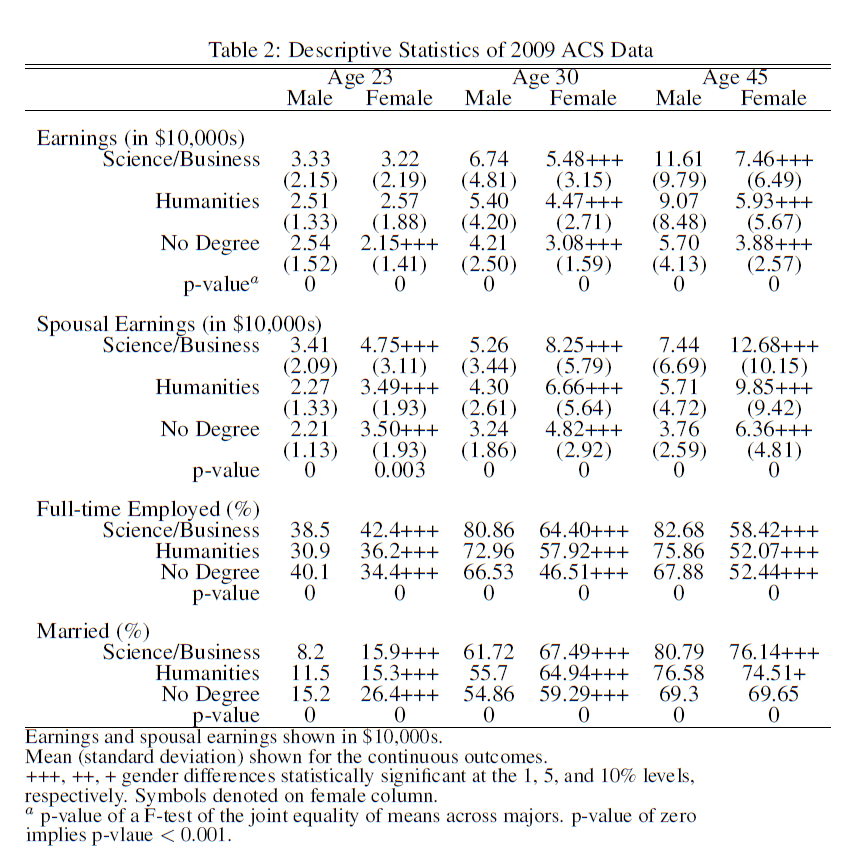
\includegraphics[scale=0.4]{Table2.png}
\end{frame}

% Earnings Beliefs: Earnings Levels
\begin{frame}{Earnings Beliefs: Earnings Levels}
    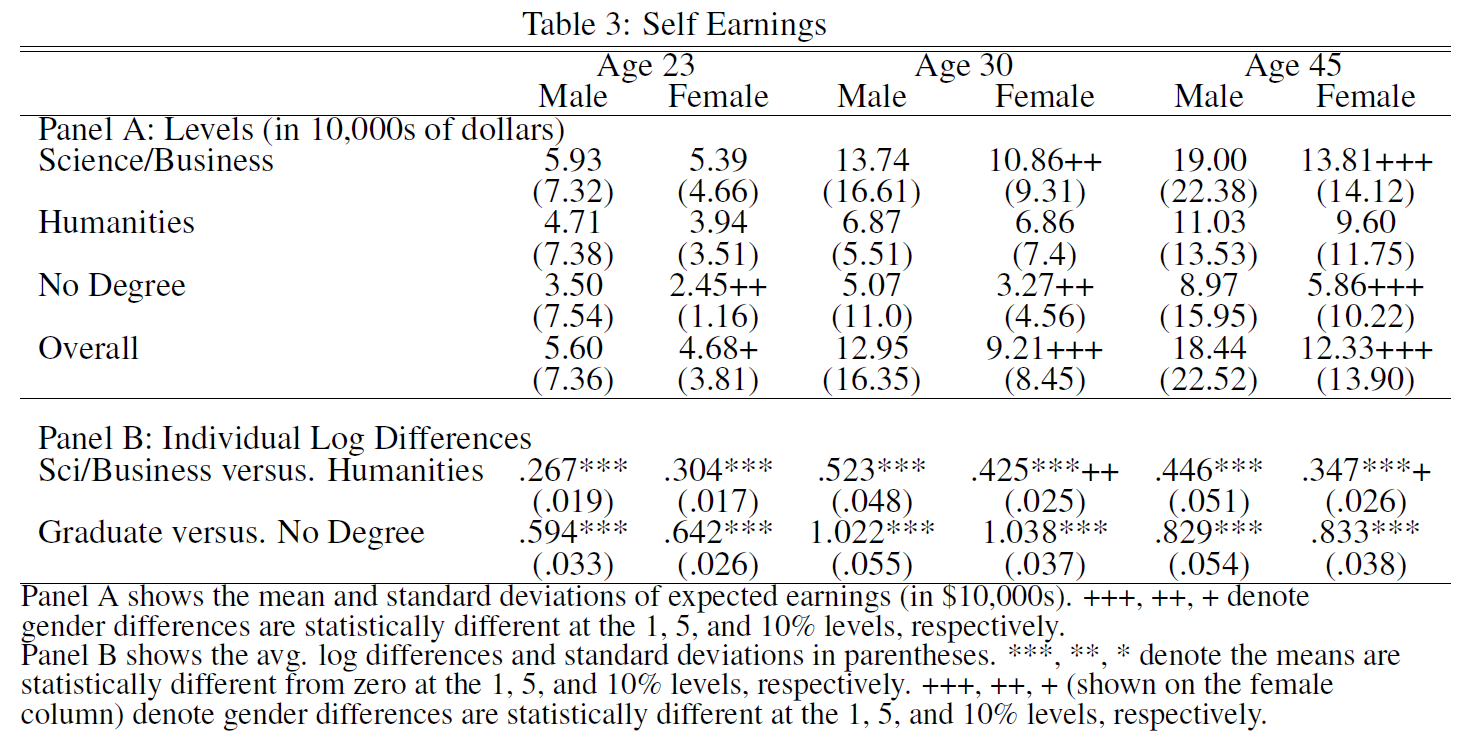
\includegraphics[scale=0.35]{Graphs/Table 3 Self Earnings.png}
\end{frame}

% Earnings Beliefs: Earnings Growth
\begin{frame}{Earnings Growth}
    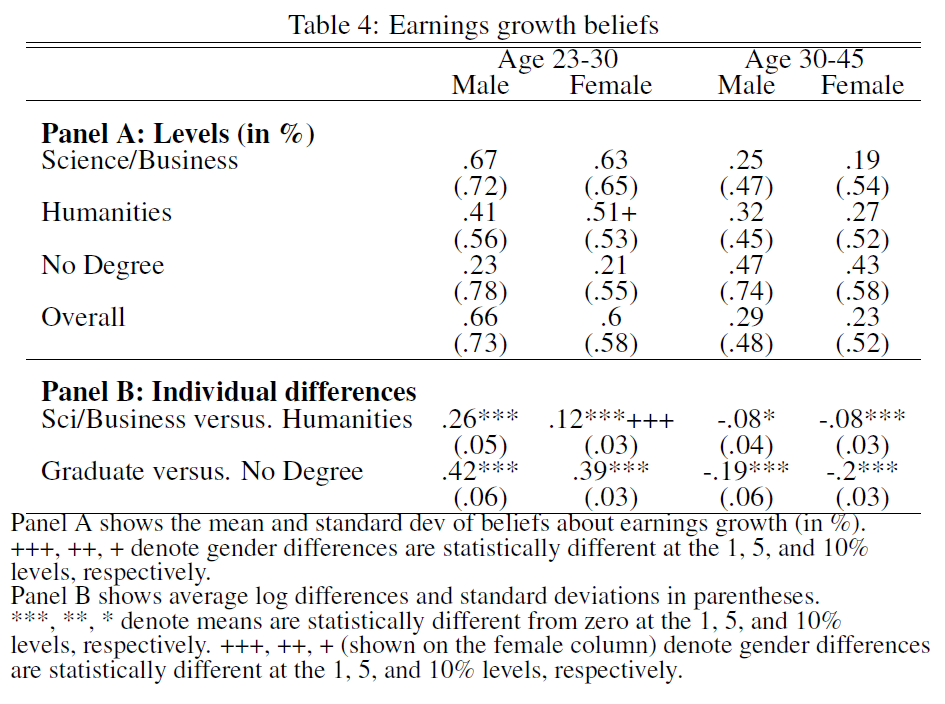
\includegraphics[scale=0.35]{Graphs/Table 4 Earnings Growth Belief.png}
\end{frame}

% Earnings Beliefs: Earnings Uncertainty
\begin{frame}{Earnings Uncertainty}
    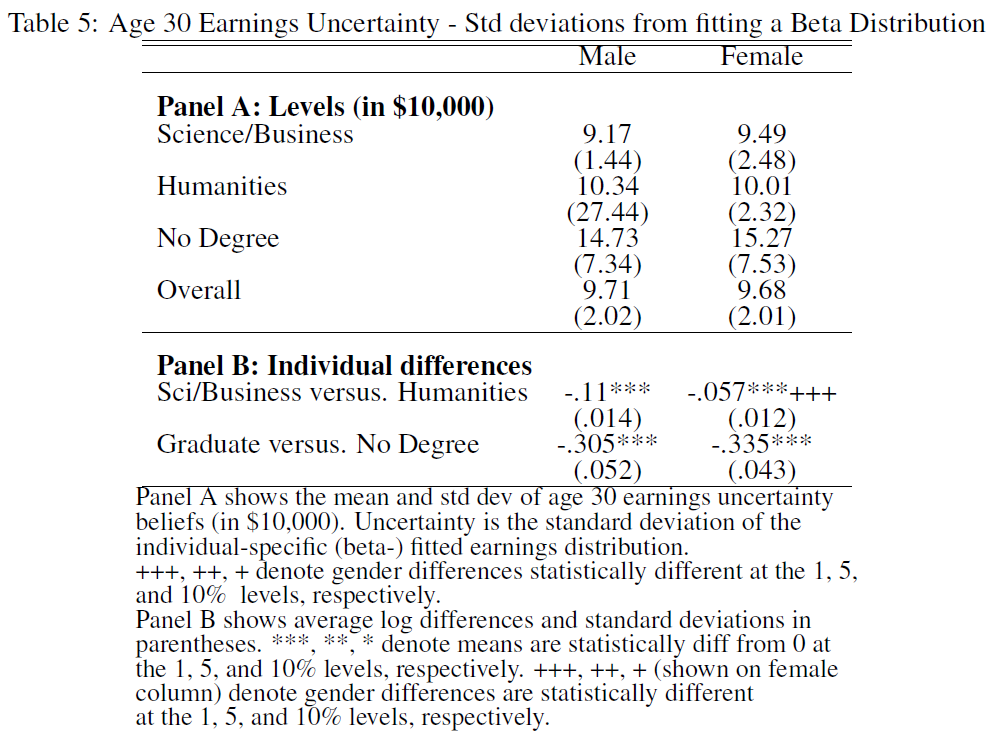
\includegraphics[scale=0.35]{Graphs/Table 5 Age 30 Earnings Uncertainty.png}
\end{frame}

% Beliefs about Marriage
\begin{frame}{Beliefs about Marriage}
    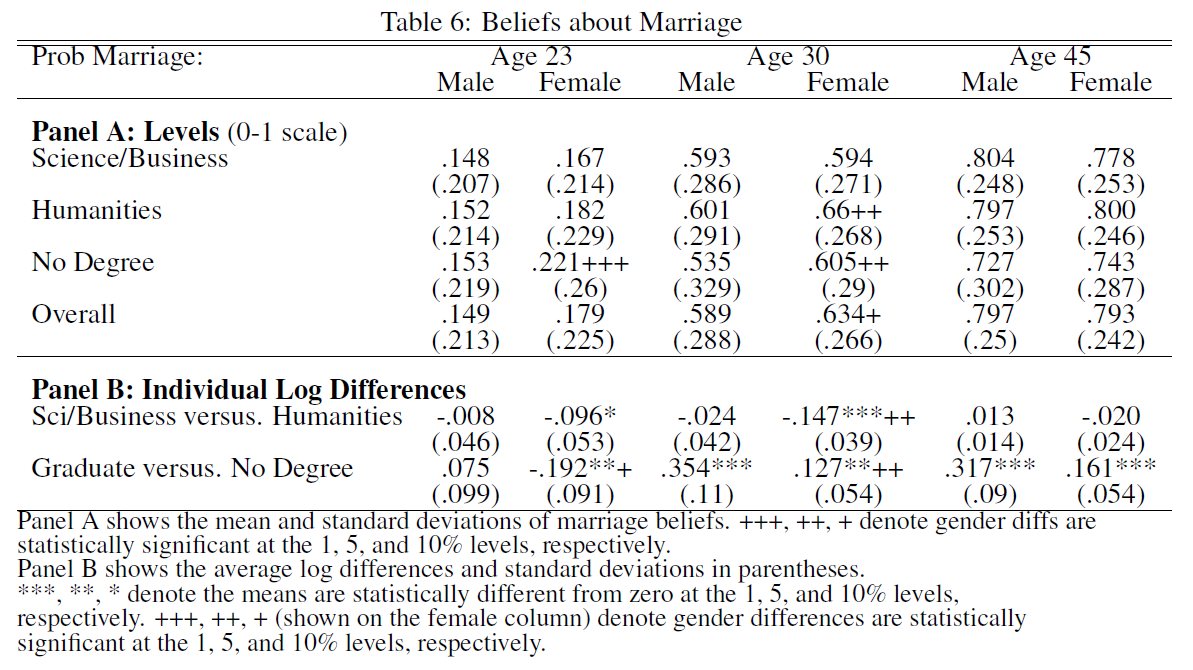
\includegraphics[scale=0.35]{Graphs/Table 6 Beliefs about Marriage.png}
\end{frame}

% Beliefs about Potential Spousal Earnings
\begin{frame}{Beliefs about Potential Spousal Earnings}
    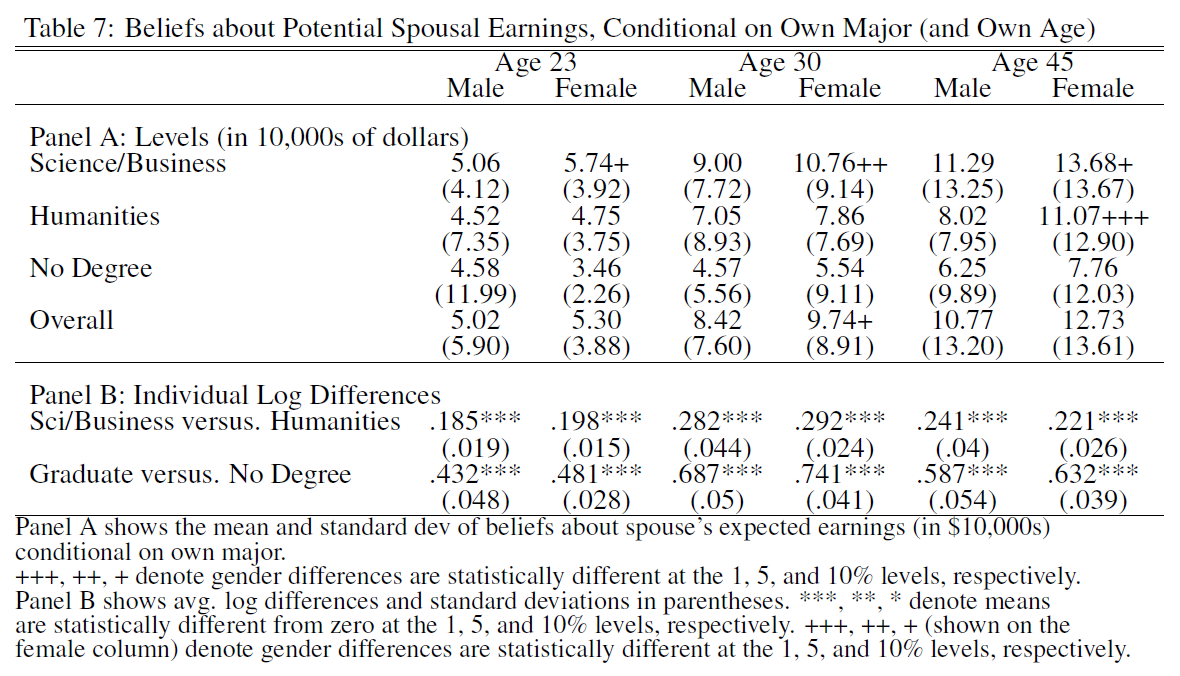
\includegraphics[scale=0.35]{Graphs/Table 7 Beliefs about Potential Spousal Earnings.png}
\end{frame}

\end{document}